%---------- Inleiding ---------------------------------------------------------

\section{Introductie}%
\label{sec:introductie}
Vandaag de dag kent sport een prominente rol bij vele Vlamingen, dat kunnen we duidelijk aflezen uit statistieken van \textcite{StatistiekVlaanderen2023} .
Hoewel sporten centraal staat voor gemiddeld \'e\'en op de vijf Vlamingen, kampt de sportsector met een sterk trainerstekort. \autocite{SportVlaanderen2023}
Met de toenemende groei van de artifici\"ele intelligentiesector ontstaat de mogelijkheid voor bijkomende hulpmiddelen om de werkdruk van trainers te verlichten.
Hierbij kunnen machine learning en objectdetectie bijdragen tot het personaliseren van een trainingsschema voor een gebruiker.
Met de opkomst van steeds slimmere AI-tools kan de drempel om te starten bovendien verlaagd worden voor startende fitnessliefhebbers.

Door de explosie aan aandacht naar artifici\"ele intelligentie en objectdetectie onstaan er mogelijkheden om nauwkeuriger resultaten te bieden aan een kleinere technologische barri\`ere.
De vraag ontstaat dan ook of fitnessclubs deze technologie\"en kunnen toepassen om het makkelijker te maken voor startende sporters en de kans op het afhaken van trainers op de lange termijn te verlagen.
Deze thesis probeert een ondersteunde oplossing te zoeken op een gebruiksvriendelijke en rendabele manier.
Zo kunnen gebruikers een fitnessschema voorgesteld krijgen door het simpelweg inscannen van de gewenste fitnessapparatuur met een mobiele telefoon.
Met machine learning kan deze apparatuur vervolgens gedetecteerd worden en kan de beginnende sporter beginnen aan zijn work-out.
Trainers kunnen makkelijk hier op voortbouwen en het trainingsschema aanvullen en hebben van in het begin een zicht op de beschikbare apparatuur.

%---------- Stand van zaken ---------------------------------------------------

\section{Literatuurstudie}%
\label{sec:state-of-the-art}

\subsection{Het ontstaan van (mobiele) AR}
\label{subsec:wat-is-ar}
Met haar eerste iteratie in de vorm van een head-mounted display ontwikkeld door \textcite{Sutherland1968} , kende Augmented Reality een opmerkelijke voorsprong op de hedendaagse smartphone.
Toch kent deze vorm van AR niet dezelfde aanneming door het algemene publiek en is tot recentelijk enkel een vorm van mobiele AR (gebruikmakend van smartphones) aanwezig op de markt.

Head-mounted AR had vooral te lijden aan grotere technologische obstakels zoals de displays waarop een samensmelting van de virtuele met de echte wereld geprojecteerd wordt \autocite{YunHan2019} .
Hierdoor was het aan koplopers zoals Meta en Varjo om aanzienlijke budgetten te besteden om deze obstakels te kunnen overbruggen en de fundamenten van deze markt tot stand te krijgen. % TODO miss bron?
Intussen zagen smartphonemakers zoals Samsung en Apple een opportuniteit om deze technologie toch in de handen te zien krijgen bij consumenten, dit in de vorm van mobiele AR.
Zo bepalen hedendaagse smartphones met behulp van camera's en sensoren de plaats van digitale entiteiten en tonen ze deze vervolgens op hun scherm.

\subsection{Head-mounted AR en gebaren}
\label{subsec:ar-gestures}
Head-mounted AR is een radicaal andere ervaring van de samensmelting van virtueel met fysiek: in tegenstelling tot mobiele AR neemt deze vorm van AR heel het gezichtsveld in beslag.
Hierdoor verdwijnt echter ook de on-screen navigatie die men vandaag de dag gewend is aan smartphones en wordt deze vervangen met gebaren.

Een mogelijk alternatief hiervoor is om via gebaren te interageren met virtuele objecten, een alternatief waar Apple vooral op zal steunen met haar Vision Pro model.
De werking hiervan wordt bepaald door middel van camera's die de posities van de gebruikers' handen bepaalt en vertaalt naar interacties met menu's \textcite{Shrestha2018} .
Uit onderzoek van \textcite{Datcu2013} blijkt dat deze manier van virtuele objecten en menu's te besturen de voorkeur kent bij gebruikers.

\subsection{Het voordeel van head-mounted devices}
\label{subsec:benefits-hmd}
Head-mounted devices maken het mogelijk voor de gebruiker om direct aan de slag te gaan met de virtuele wereld zonder hierbij een telefoon vast te houden.
Het gevoel van kijken door een soort venster verdwijnt doordat de samensmeltende werelden direct geprojecteerd worden in de ogen van gebruikers.
Deze categorie van AR-apparaten krijgt daardoor vaak de term \("\)Immersive AR\("\) en kent ook vandaag al een meerwaarde in onder andere de medische sector tijdens het opleiden van chirurgen~\autocite{Waisberg2023} .

%---------- Methodologie ------------------------------------------------------
\section{Methodologie}%
\label{sec:methodologie}
\subsection{Voorafgaande literatuurstudie}
\label{subsec:literature-study}
In de eerste fase vindt zich een voorafgaande literatuurstudie over het onderwerp plaats. % 3 weken
Het praktische doel hiervan is om een verdere inzicht te krijgen op de werking van machine learning en haar rol bij object detectie op foto's.
De nadruk ligt hierbij op de evolutie van deze werking en de verschillen tussen lokale machine learning applicaties en die van cloudproviders zoals Amazon en Google.
Tijdens deze fase komen de gelijkenissen en verschillen tussen de twee varianten aan bod om tijdens de derde fase te kunnen vergelijken aan de hand van een proof-of-concept.

\subsection{Dataverzameling}
\label{subsec:dataverzameling}
Vervolgens vindt er zich een requirements-analyse plaats om af te toetsen waar de focus moet liggen bij objectdetectie. % 3 weken
Gebruikers die een app gebruikmakend van deze tool wensen te gebruiken tijdens het sporten horen eender welke gerelateerde apparatuur in te kunnen scannen.
Om dit te realiseren moet de dataset getraind worden op gepaste en gevarieerde fitnessapparatuur in verschillende fitnessclubs.
Hiervoor wordt data in de vorm van foto's en beschrijvingen verzameld, gepaard met de gebruiksmogelijkheden en eventuele advies van trainers.
Dit wordt vervolgens gegoten in bruikbare datasets in de derde fase.
Ook zal hiermee de mogelijkheid ontstaan voor gebruikers om een gepersonaliseerd fitnessschema aan te bieden, deels vooropgesteld door trainers.

\subsection{Proof-of-concept}
\label{subsec:poc}
Gedurende de derde fase wordt een proof-of-concept applicatie gebouwd voor Android-apparaten. % 4 weken
Hiervoor worden er eerst datasets gegenereerd voor de objectdetectie functionaliteit.
Deze datasets zullen enerzijds gebruik kunnen maken van de machine learning capaciteiten van Google Cloud (Vertex AI) of anderzijds gegenereerd worden op een lokale computer gebruikmakend van het Tensorflow framework.
Hiermee kunnen we het verschil in kwaliteit testen om vervolgens de waarde van de platformen af te toetsen tegenover de kostprijs.
De proof-of-concept toetst de mogelijke antwoorden die tijdens de literatuurstudie aan bod kwamen op de requirements af.

\subsection{Rapport met aanbevelingen}
\label{subsec:result-of-poc}
Na het opzetten van de proof-of-concept komen enkele gebruikerstests aan bod. % 3 weken
Hierbij worden het gebruikspatroon, de tijdsduur en foutenpercentage van objectdetectie vastgelegd.
Een analyse van deze cijfers zal de bruikbaarheid van het gebruiken van objectdetectie en genereren van gepersonaliseerde trainingsschema's aantonen.
Daaropvolgend wordt een rapport met aanbevelingen opgesteld voor ontwikkelaars die soortgelijke functies willen implementeren.
Belangrijk hierbij is dat ontwikkelaars dit rapport kunnen gebruiken om te kunnen kiezen tussen een lokaal gegenereerde dataset of gebruikmakend van clouddiensten zoals Google Cloud.

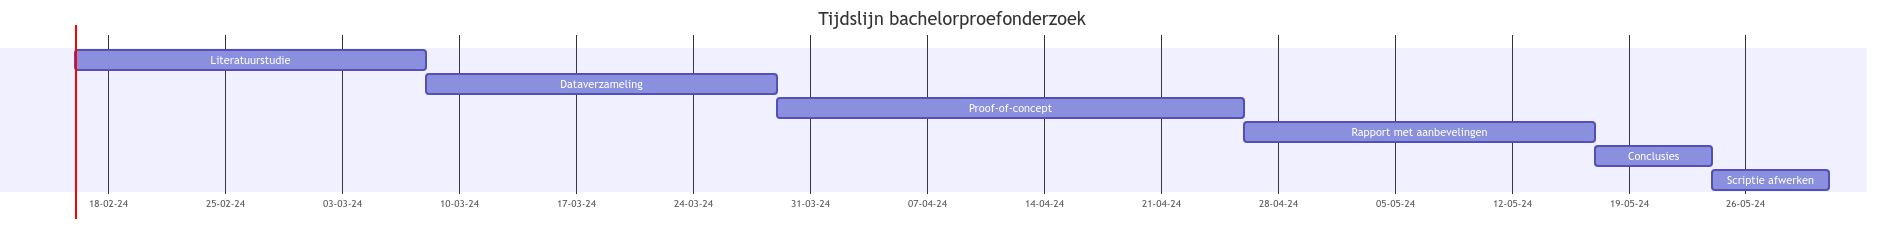
\includegraphics[width=0.5\textwidth]{ganttChart}

%---------- Verwachte resultaten ----------------------------------------------
\section{Verwacht resultaten en conclusie}
\label{sec:verwacht-resultaten-en-conclusie}
Er wordt verwacht dat de resultaten uit de proof-of-concept zal leiden tot een bruikbare tool die de drempel tot het starten van sport verlagen.
Deze tool zal concreet de mogelijkheid bieden om fitness apparatuur in te scannen en detecteren door middel van machine learning.
Hiermee kunnen ontwikkelaars die werken voor fitnessketens snel aan de slag voor gepersonaliseerde applicaties.
De hypothese stelt dat de drempel om te starten in een fitnessclub zal verlaagd worden en dat coaches meer kunnen focussen op langetermijnschema's.
Aan de hand van het aanbevelingsrapport kunnen ontwikkelaars ervoor kiezen om gebruik te maken van Google Cloud voor nauwkeurigere oplossingen of voor een lokale machine voor een lagere kostprijs.